%\documentclass[12pt,a4paper]{IEEEtran}
\documentclass[12pt,a4paper]{article}
\usepackage{lmodern}
\usepackage[utf8]{inputenc}
\usepackage[english]{babel}
\usepackage{amsmath}
%\usepackage{amsfonts}
\usepackage{graphicx}
\usepackage{amssymb}
\usepackage{csquotes}
%\usepackage[left=2cm,right=2cm,top=2cm,bottom=2cm]{geometry}
\usepackage[backend=biber]{biblatex}
\bibliography{references}
\author{Schwarenthorer Yannick, 1229026}
\title{\vspace{-3cm}Password meters}
%\title{Password meters}

\begin{document}

\maketitle


\section*{Abstract}
\label{sec:abstract}
This summary is looking at password meters and the effectiveness of them.
We will compare some of the most used password meters of Apple, eBay and Google. 
In section 5. we will look into the details of how one of the currrent best meters (zxcvbn) from dropbox works. Additionally the paper  \citetitle{differentapproaches} will summarize our explanations and give further insights.

%differentapproaches

%\tableofcontents 

\section{Introduction}
\label{sec:introduction}
Passwords are still the main authentication mechanism on all kinds of systems and according to the leading tech society they will be with us for at least 10 years.
The security and privacy of all our data relies on a human generated string of characters and numbers.
This rich structure makes them a target of guessing attacks. Therefore we must nudge the user to create harder to guess passwords.

\section{Effect of password meters}

\label{sec:effect}
In this section we will take a look at the effect of password meters.
In the paper \citetitle{upToEleven} \cite{upToEleven} the authors show that the present of a password meter has an effect on the password strength. However this holds only for sites which the users rated as important. For lower risk websites (sites which store no personal information about the user) the password strength is not higher when a password meter is present.

%Other papers: users allways aware that there password is tested -> not so good data then

\subsection{Experiments}
The authors of the paper performed two experiments, the first one aims to show that the presence of a password meter has an effect on the password strength. The second field experiment tests if the importance of the site on which the meter is present has an influence on the result.

% 1: Examine wheteever meters influence password strength of users.
%1) When the changed there real password
%2) When the were not told that their password will be examined

\paragraph{Laboratory experiment} 

The participants were forced to change their real university network password while evaluating the usability of a new user interface, therefore the users were not aware that their password strength is the object of a study. In the laboratory experiment they tested following hypotheses:
\begin{itemize}
    \item [$ H _{0}$]: Passwords are not stronger when meters are present.
    \item [$ H _{1}$]: Passwords are stronger when users see relative strength meters	compared to no meters.
    \item [$ H _{2}$]: Passwords are stronger when users see relative strength meters compared to "traditional" meters.
\end{itemize} 
All together they tested 47 participants changing their real passwords. With the help of a proxy server they collected the data and calculated the relative strength of the passwords in bits of entropy. The relative strength meter mentioned in the hypotheses $ H _{1}$ and $ H _{2}$ are based on social pressure. The meter displays the percentage of users which have a stronger password than the currently chosen one. The 47 users get assigned randomly to one of three groups: 

\begin{enumerate}
	\item Traditional password meter with "weak", "medium" or "strong" ratings. In short terms: existing motivator (EM)
	\item Strength relative to all of the other users on the system: peer pressure motivator (PPM)
	\item Control group with no password meter
\end{enumerate}

%Traditional meters (weak, medium, strong) --> existing motivator (EM) 
%and
%(social pressure) strength relative to all of the other user on the system. (peer pressure motivator (PPM)).
%Random assigment to one of three groups --> EM,PPM or control condition with no meter.
%only relative diffrents between the password strength! 
%hange of password of university site, proxy for collecting data, not stored real password!

\paragraph{Results}
Both password meters led to statistically significant differences, when compared to the control group. At the beginning, the passwords where all 46.7 bits strong. In the EM condition the entropy of the chosen passwords have raised to 60.8 (p $<$ 0.001). In the PPM condition the entropy raised to 64.9 bits (p $<$ 0.008). 
When compared to the control group they can reject $H _{0}$ and accept $H _{1}$.
The difference between the traditional meter and the "peer-pressure-motivator" is not significant enough to accept $H _{2}$.

\paragraph{Field experiment} 

In the followed field experiment 200 participants created a password for an unimportant account. 
They tested following null hypothesis:
\begin{itemize}
    \item [$ H _{0a}$]: Passwords are not stronger, when users see meters, when creating unimportant accounts.
    \item [$ H _{0b}$]: Changes to the orientation and text of password meters will not result in different passwords.
\end{itemize} 
They designed the experiment so that they can measure the effectiveness off traditional meters (EM) and social pressure meters (PPM) while controlling for meter orientation.

%eight different experimental conditions, so that they can control three different factors: meter orientation (horizontal or vertical), meter meaning (weak/strong or based on social pressure), and the different between text and graphical strength feedback.

\paragraph{Results}
They did not find statistically significant differences between the conditions. Therefore they could not reject either $ H _{0a}$ or $ H _{0b}$. Compared to the laboratory result, they concluded that the users did not choose a stronger password because of the unimportance of the side on which they had to choose a password.

\section{Effect of password meters on predictability }

In the paper \citetitle{measureUp} \cite{measureUp} the authors take another approach for testing the effects of password meters. They tested the predictability of passwords with common password cracking tools like "john the riper" on user generated passwords with and without password meters. They measured the predictability with a guess-number calculator, which calculates how many guesses a cracking algorithm will need, to crack a given password without running the algorithm.
They used Amazon's mechanical Turk for requiring participants. They tested their own password meter in 14 different variations of strictness and so on. They also added a control group with no meter.

\paragraph{Experiment}
The 2931 people acquired from the mechanical Turk, were randomly assigned to one of the 14 variations of the creation page of a fake e-mail provider.
Those 14 version are basically a variation of different feedback types for the strength of a password, ranging from simple text feedbacks up to animated cartoon characters. The authors then tried to calculate the predictability of the password as described above. They considered three attacker scenarios. The weak attacker with limited computational resources, which can make up to 500 million guesses. The medium attacker with 50 billion guesses and in the strong attacker scenario they would calculate how many passwords will be cracked in the first 5 trillion (5 x $10^{12}$) guesses.

%John the Ripper4, a popu- lar password cracker, can crack 500 million hashed pass- words in about an hour on a modern desktop machine. Five trillion guesses would require a botnet of several hundred machines working for several days.

\paragraph{Results}
The presence of any password meter (expect the text-only one) increased the password length. In conditions where the meter is very stringent, it also increases the use of digits and symbols. 
As shown in figure 1, in terms of password predictability, each password meter has a slightly better result against all three attack scenarios compared to no meter. Although not all of the results were statistically significant. The two very stringent meters with visual bars performed best. Those meters (one-third-score and half-score) are just downgrading each password strength score of the base line meter with the factor 1/2 and 1/3. On the downside, these meters led participants to believe that they calculate the score wrong and therefore place less attention to them.

\begin{center}
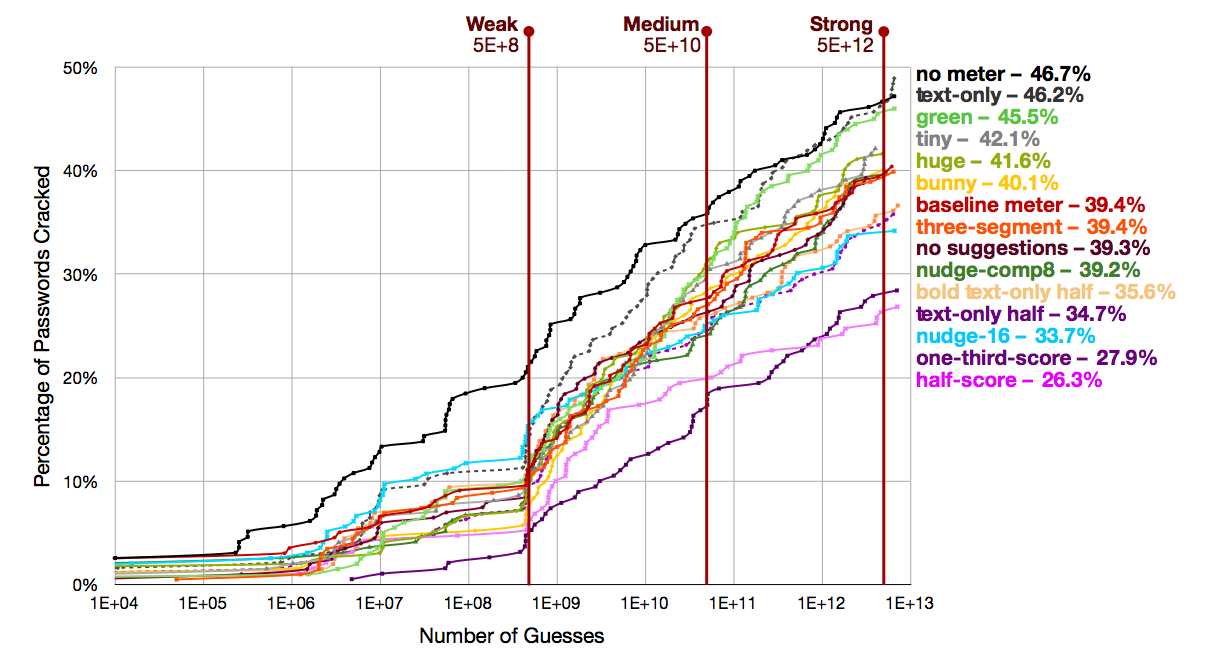
\includegraphics[height=8cm]{percentageOfPasswordsCracked}
Figure 1  \cite{measureUp}
\end{center}

\section{Comparison}
\label{sec:Comparison}
In this section we will compare some password meters from commonly known websites. We will explain briefly how they work internally. This section is inspired by the paper \citetitle{weakToStrong} \cite{weakToStrong}. 
The authors tested 11 prominent web service providers. The results are in a wide range from not understandable (yahoo) to very good (dropbox).

\paragraph{Google}
Google implements the same hybrid checker on all of its websites. After the minimum length requirement of 8 characters is fulfilled, the password is send to a server for further evaluation.
For some passwords google acts very inconsistent. For example testtest is weak, testtest0 is strong, testtest1 is fair, testtest2 is good and testtest3 is strong again. Such behaviour is confusing and frustrating for the user, since he cannot understand the calculations. Furthermore, the strength of a password can vary from time to time, even in a few minutes one can get different results for the same password.
The worst facts are implementation error, where deleting and re-entering the same character from a correct password leads to an "to short" password.

\paragraph{eBay}
Ebay uses a fully server side checker. Other than Google, they also check for the usage of the entered username or similar. The algorithm itself is very simple and was nearly recreated by the authors with 20 lines of javascript-code. The password length becomes irrelevant once it is beyond the minimum of 8. After that the password meter only counts the used character classes. It seems that eBay does not make any dictionary lookups, since for example the very simple password "P@ssw0rd" is marked as strong.

\paragraph{Apple}
They have implemented a hybrid checker similar to Google. Once the client side requirements are met, the password is sent to a server for further checking, including a very strict blacklist check. These blacklisted passwords are disallowed, irrespective of the measurements of the client side checker. This client side checker calculates an increasing only score. The score is better if a password is longer and contains at least an uppercase letter, a symbol and one ore more digits. Strangely a password can be rated as strong an still be rejected because not fulfilling all requirements.

\paragraph{Dropbox}
Dropbox is the only one which explains their design choices in detail. See chapter 5. for more information about their algorithm called "zxcvbn".

%\subsection{Evaluation Framework}
%Evaluation Framework --> 
%- no harder than LUDS to adopt
%- should estimate guessing order
%- accurate at low magnitudes
%- adjustable size



%
%
% ZXCVBN
%
%

\section{Zxcvbn}
\label{sec:zxcvbn}
Zxcvbn is an open sourced password meter developed from Dropbox inc. It checks how common a password is and how easily it can be guessed by an attacker. Therefore it calculates heuristically how much attempts an attacker would need to guess the password. To achieve this, zxcvbn separates the work in three phases: match, estimate and search. A simple example would be a password with 2 words from top100 common password list, zxcvbn will calculate $ 100^{2} $ guesses for such a password. The algorithm assumes that the attacker knows the patterns that make up the password, but not how many or in which order.

%TODO welche password dumps werden verwendet

%The older 2012 version has some differents comparing to the 2016 version:comparision 2012 vs 2016 version, jessiah03 (Seite. 162, links oben)

\subsection{Matching}
In this phase the algorithm matches patterns to a given plaintext password. 
It finds a set of overlapping matches. Zxcvbn will match the following patterns: tokens, reversed words, sequences, dates, repeats, keyboard patterns and brute-force sections. For the password 'lenovo1111' the matching phase will find the patterns: lenovo (common word), eno, one (english dictionary), no (english dictionaray), on (english dictionary or reversed no), 1111(repeat), 1111(date)

%Table! List of patterns:
%- token: 
%- reversed
%- sequence
%- bruteforce
%- date
%- repeat
%- keyboard

\paragraph{Token matcher} 

This pattern matcher lowercases the password and checks each substring against a frequency-ranked dictionary. 
Additionally, a transformation for common l33t-translations is made based on a l33t-Table which maps equal looking characters to their counterpart.
With this approach it is possible that the matcher can detect the base password 'logitech' from the leeted version 'l0giT3CH'.
%l33t-Table: @->a, e->3 etc. if two possibles each is tested.

\paragraph{Repeat matcher}
The repeat matcher looks for repeated blocks of one or more characters.
This matching is proceeded recursively on a winning unit, so it is also possible to identify repeated dictionary words or dates.

%(Rewrite of 2012 version which only single character repeats)
%examples: greedy and lazy regex
%greedy beats lazy for aabaab recognizing aab over the full string vs a repeated over aa. lazy beats greedy for aaaaa, matching a spanning 5 characters vs aa spanning 4..
%matching recursively on winning unit --> identification of repeated words and dates.

\paragraph{Keyboard matcher}
Here zxcvbn looks for keyboard patterns. The matcher runs through the password and looks up the keystrokes in a graph of keyboard layouts. This graphs represents each key on a specific keyboard layout, connecting them to their neighbours. The matcher than counts the chain length, number of turns and number of shifted characters.

%This  Keyboard matching is runs throw password linear, looking for keyboard patterns, graph of keyboard layout! qwerty dvorak etc. included by default. others can be added. 
%Keyboard key graph are mappings "between each key to a clockwise positional list of its neighbours." "matcher counts chain length, number of turns, and number of shifted characters"

\paragraph{Date matcher}
%4-8 characters.
This pattern matcher looks for dates in the password. It analyses each substring of the length of 4 up to 8 characters and checks in a table for possible splits. Each split is analysed separately with some given constraints. E.g. the year is 2 or 4 digits and not in the middle, the month is between 1-12 and the day between 1 and 31 (inclusive). 
For example the string "201689" has 3 candidates. First 20-16-89 which is a invalid month, second 2-0-1689 where 0 is an invalid day or month and finally the best one 2016-8-9. If multiple dates are correct the one nearest to the reference year 2016 is chosen. Similar two digit years are matched to the 20th or 21th century depending on which is closer to 2016. For simplicity zxcvbn doesn't look for improper dates like the 29. Februrary on a non leap year.

%- checks table for possible splits
%- tries day-month-year mapping for each split: 
%	year is 2 or 4 digits and not in the middle. month between 1-12, day between 1 and 31 inclusive.

%examples: "201689" -->
%- 2016-8-9 --> best one
%- 20-16-89 --> invalid month
%- 2-0-1689 --> 0 is invalid for month and day

%If multiple dates are correct, date which is closest to year 2016 wins!

%Two digit years are matched to 20th or 21th century depending on which is closer to 2016

%No filtering of inproper dates like 29.feb on non leap year

\subsection{Estimation}

In this phase the algorithm assigns a guess attempt to each match from the previous matching phase.
Zxcvbn uses following heuristic for the estimation: "if an attacker knows the pattern, how many guesses might they need to guess the instance?" \cite{zxcvbn}. For example the previous password "lenovo" is ranked 11007th in on of the used password dictionaries. Therefore it gets assigned a score of 11007 because an attacker would try it as the 11007 one. In general it is assumed that an guesser will attempt simpler more likely patterns first.

\paragraph{Tokens}
As stated above, on tokens the frequency rank in a password dictionary is used as estimation. For Reversed tokens the guesses will be doubled since the attacker has to guess both directions of each word. The result gets doubled if the password has obvious s uppercase letters (first-character, last-character or all characters). Otherwise capitalization factor is calculated width this formula:

\begin{center} $ \dfrac{1}{2} \sum\limits_{i=1}^{min(U,L)} \binom{U+L}{i} $ \end{center}

U and L are the number of upper and lowercase letters in the token. The 1/2 term converts the total guessing space to an average attempts needed.

%\paragraph{Guesses for Keyboard patterns}
%\paragraph{Repeat match}
%\paragraph{Bruteforce matches}

\subsection{Search}

In this phase zxcvbn is searching for sequences of non-overlapping adjacent matches, so that the password is covert and total guess attempts are minimized. For example in the "lenovo1111" password the "1-1-11" date pattern gets discarded because it requires more guesses than the repeat pattern.

\subsection{Result}
As a result of all the calculations zxcvbn can calculate the guesses needed for an attacker for a given password. The developer who implements the algorithm on his own website can now decide how stringent the password meter should be, by giving a number of minimum guesses the password should survive during a guessing attack. This gives the perfect ability for trading of password security with the usability of the password choosing process.

%search heuristic, (formel (1) ), soll die rein?

\section{Conclusion}
Password policies and password meters seem to be the way to go until we find a replacement for passwords.
As stated in \citetitle{differentapproaches} \cite{differentapproaches}, password meters in general help users with the creating of a better password. "Most users did not feel annoyed using a password strength meter." \cite{differentapproaches}. This quote can be interpreted in a way, that password security has to be carefully traded of with the usability. Because the last thing a system administrator wants is a user who is writing his passwords done on a piece of paper or heavily reuses them.

\printbibliography

\end{document}
